\documentclass[12pt,handout]{beamer}

%\documentclass{beamer}
\usetheme{Boadilla}
\useoutertheme{split}
\usepackage{fancyvrb}
\usepackage{tikz}
\usepackage{svg}
\usetikzlibrary{shapes, calc, shapes, arrows, datavisualization}

\usepackage{amsmath,amssymb}

\definecolor{myblue}{RGB}{80,80,160}
\definecolor{exerciseblue}{RGB}{200, 200, 247}
\definecolor{mygreen}{RGB}{80,160,80}


\title{Getting Started with Gurobi}
\author{Abr\'emod Training}
\titlegraphic{
\includegraphics[scale=0.1]{abremodlogo.png}}


\begin{document}

\begin{frame}
\titlepage
\end{frame}

\begin{frame}
\frametitle{Overview}
\begin{itemize}
\item Linear Programming (LP)
\item Solving LPs with Gurobi
    \begin{itemize}
    \item Interactive Shell (Python)
    \end{itemize}
\item LP Modeling Techniques
\item Multi-Objective Optimization
\item Integer Programming
\item Performance Tuning
\item Column Generation
\item Convex Quadratic Programming
\item Stochastic Programming
\end{itemize}
\end{frame}

\begin{frame}
  \frametitle{Abr\'emod}
Abr\'emod specializes in implementing math programming models to solve business problems.
Including business analysis, modeling, and implementation.
\begin{itemize}
\item Revenue Management
\item Assignment/Scheduling Problems
\item Network Optimization
\end{itemize}
\end{frame}

\begin{frame}
\frametitle{Gurobi}
Gurobi is a state-of-the-art solver for mathematical programming. It includes solvers for the following types of models:
\begin{itemize}
\item Linear Programming (LP)
\item Mixed-Integer Linear Programming (MILP)
\item Quadratic Programming (QP)
\item Mixed-Integer Quadratic Programming (MIQP)
\item Quadratically Constrained Programming (QCP)
\item Mixed-Integer Quadratically Constrained Programming (MIQCP)
\end{itemize}
Here, ``program'' does not refer to a computer program but rather a schedule.
\end{frame}

\begin{frame}
\frametitle{Gurobi}
\begin{itemize}
\item The problems Gurobi solves are all special cases of mathematical programs.
\item Before we discuss those special cases in detail, we should understand what a math program looks like and define some related terminology.
\end{itemize}
\end{frame}

\begin{frame}
\frametitle{What is a Mathematical Program?}
A math program consists of three components:
\begin{itemize}
\item Decision Variables (what you control)
\item Constraints (rules you must follow)
\item Objective Function (what you want to minimize/maximize)
\end{itemize}
\end{frame}

\begin{frame}
\frametitle{What is a Mathematical Program?}
\begin{block}<+->{Definition}
%\begin{align*}
\begin{eqnarray}
\mbox{minimize/maximize:} && f(x_1, x_2, \ldots, x_n) \nonumber \\
\mbox{subject to:} && g_i(x_1, x_2, \ldots, x_n)
\begin{Bmatrix}   \le \\
                   \ge \\
                   =
\end{Bmatrix}
b_i, \;\; i = 1, \ldots, m \nonumber \\
&& x_j \ge 0,\;\;j = 1, \ldots, n \nonumber
\end{eqnarray}
%\end{align*}
\end{block}
\end{frame}

\begin{frame}
\frametitle{Math Programming Terminology}
\begin{itemize}
\item $x_j$ are the {\em decision variables}.
\item $g_i(x_1, x_2, \ldots, x_n) \begin{Bmatrix}   \le \\
                    \ge \\
                    =
\end{Bmatrix} b_i$ are {\em structural constraints}.
\item $x_j \ge 0$ are {\em nonnegativity constraints}.
\item $f(x_1, \ldots, x_n)$ is the {\em objective function}.
\item A {\em feasible solution}, $\hat{x} = (\hat{x}_1, \ldots, \hat{x}_n)$ satisfies all constraints.
\item The {\em feasible region} is the set of all feasible solutions.
\item The objective function ranks the feasible solutions.
\item The optimal solution $x^*$ satisfies $f(x^*) \le f(\hat{x})$ for all feasible $\hat{x}$.
\begin{itemize}
\item $x^*$ is feasible itself.
\end{itemize}
\end{itemize}
\end{frame}

\begin{frame}
\frametitle{The Linear Program}
\begin{eqnarray}
z^* = \min_x && c_1 x_1 + c_2 x_2 + \cdots + c_n x_n \nonumber \\
\mbox{subject to:} &&a_{i1} x_1 + a_{i2} x_2 + \cdots + a_{in} x_n
\begin{Bmatrix}   \le \\
                   \ge \\
                    =
\end{Bmatrix}
b_i,\;\;i = 1,\ldots,m \nonumber \\
&&x_1, x_2, \ldots, x_n \ge 0 \nonumber
\end{eqnarray}
In standard matrix form:
\begin{eqnarray}
z^* = \min_{x} && c^T x \nonumber \\
\mbox{s.t.} && Ax = b \nonumber \\
&& x \ge 0 \nonumber
\end{eqnarray}
\end{frame}

\begin{frame}
\frametitle{The Linear Program}
\begin{eqnarray}
z^* = \min_x && c_1 x_1 + c_2 x_2 + \cdots + c_n x_n \nonumber \\
\mbox{subject to:} &&a_{i1} x_1 + a_{i2} x_2 + \cdots + a_{in} x_n
\begin{Bmatrix}   \le \\
                   \ge \\
                    =
\end{Bmatrix}
b_i,\;\;i = 1,\ldots,m \nonumber \\
&&x_1, x_2, \ldots, x_n \ge 0 \nonumber
\end{eqnarray}
\begin{itemize}
\item $a_{ij}$, $c_j$, and $b_i$ are data.
\item Find $x^*$ satisfying $c_1 x_1^* + \cdots + c_n x_n^* \le c_1 \hat{x}_1 + \cdots + c_n \hat{x}_n$ for all feasible $\hat{x}$.
\item A linear program (LP) is a special type of math program with:
    \begin{itemize}
    \item $f(x_1,\ldots,x_n) = c_1 x_1 + \cdots + c_n x_n$
    \item $g_i(x_1,\ldots,x_n) = a_{i1} x_1 + \cdots + a_{in} x_n,\;\;i = 1,\ldots,m$
    \end{itemize}
\end{itemize}
\end{frame}

\begin{frame}
\frametitle{Linear Programming Axioms}
\begin{eqnarray}
z^* = \min_x && c_1 x_1 + c_2 x_2 + \cdots + c_n x_n \nonumber \\
\mbox{subject to:} &&a_{i1} x_1 + a_{i2} x_2 + \cdots + a_{in} x_n
\begin{Bmatrix}   \le \\
                   \ge \\
                    =
\end{Bmatrix}
b_i,\;\;i = 1,\ldots,m \nonumber \\
&&x_1, x_2, \ldots, x_n \ge 0 \nonumber
\end{eqnarray}
\begin{itemize}
\item Additivity
\item Proportionality
\item Divisibility
\item Certainty
\end{itemize}
\end{frame}

\begin{frame}
\frametitle{Linear Programming Transformations}
Gurobi will automatically perform the following transformations to get into standard form:
\begin{itemize}
\item Maximize by minimizing the negative
    \begin{itemize}
    \item $\max_x cx \Leftrightarrow \min_x -cx$
    \end{itemize}
\item Add a slack or surplus variable to convert inequality into equality
    \begin{itemize}
    \item $ax \ge b \Leftrightarrow ax - s = b, s \ge 0$
    \item $ax \le b \Leftrightarrow ax + s = b, s \ge 0$
    \end{itemize}
\item Write a variable that can be positive or negative as the difference of non-negative variables
    \begin{itemize}
    \item $x = x^+ - x^-$
    \item $x^+, x^- \ge 0$
    \end{itemize}
\end{itemize}
\end{frame}

\begin{frame}
\frametitle{The Diet Problem}
\begin{itemize}
\item Suppose you are trying to construct a diet out of a given set of foods, each with a different cost and nutritional composition, and wish to meet some minimum requirements of various nutrients.
\item How can you find the combination of foods that meets all the nutrient requirements and minimizes cost?
\end{itemize}
\end{frame}

\begin{frame}
\frametitle{The Diet Problem}
Let's consider the following sample inputs where there are 5 types of food and 2 nutrient requirements.
\begin{center}
Units of nutrients and cost per ounce
\begin{tabular} {c | c | c | c}
Food type & Iron & Calcium & Cost \\
\hline
1 & 2 & 0 & 20 \\
2 & 0 & 1 & 10 \\
3 & 3 & 2 & 31 \\
4 & 1 & 2 & 11 \\
5 & 2 & 1 & 12 \\
\end{tabular}
\end{center}
Nutrient requirements: 21 units of iron and 12 units of calcium
\end{frame}

\begin{frame}
\frametitle{Diet Problem Formulation}
\begin{columns}[t]
\begin{column}{5cm}
\begin{center}
\begin{tabular} {c | c | c | c}
Food & Iron & Calcium & Cost \\
\hline
1 & 2 & 0 & 20 \\
2 & 0 & 1 & 10 \\
3 & 3 & 2 & 31 \\
4 & 1 & 2 & 11 \\
5 & 2 & 1 & 12 \\
\end{tabular}
\end{center}
Nutrient requirements: \\ Iron: 21, Calcium: 12
\end{column}
\begin{column}{7cm}
\begin{itemize}
\item Decision Variables
    \begin{itemize}
    \item $x_j = $ \# of ounces of food type $j = 1, 2, \ldots, 5$
    \end{itemize}
\item Objective Function
    \begin{itemize}
    \item min $z = 20 x_1 + 10 x_2 + 31 x_3 + 11 x_4 + 12 x_5$
    \end{itemize}
\item Structural Constraints
    \begin{itemize}
    \item $2 x_1 + 0 x_2 + 3 x_3 + 1 x_4 + 2 x_5 \ge 21$
    \item $0 x_1 + 1 x_2 + 2 x_3 + 2 x_4 + 1 x_5 \ge 12$
    \end{itemize}
\item Nonnegativity constraints
    \begin{itemize}
    \item $x_j \ge 0, j = 1, 2, \ldots, 5$
    \end{itemize}
\end{itemize}
\end{column}
\end{columns}
\end{frame}


\begin{frame}
\frametitle{Solving with the Gurobi Interactive Shell}
\begin{itemize}
\item Objects and Methods you will need
    \begin{itemize}
    \item Model
        \begin{itemize}
        \item addVar(lb, ub, obj, vtype, name)
        \item addConstr(constr, name)
        \item update()
        \item optimize()
        \end{itemize}
    \item Var
        \begin{itemize}
        \item X
        \item RC
        \end{itemize}
    \item Constr
        \begin{itemize}
        \item Pi
        \item Slack
        \end{itemize}
    \end{itemize}
\end{itemize}
\end{frame}

\begin{frame}
\frametitle{Querying the Solution}
\begin{itemize}
\item Model.write()
    \begin{itemize}
    \item m.write(`diet.lp') outputs the model in human-readable form
    \item m.write(`diet.mps') outputs a full-precision copy of the model
    \item m.write(`diet.sol') outputs the solution
    \end{itemize}
\item Model object attributes
    \begin{itemize}
    \item m.Status (was the solver able to find an optimal solution?)
    \item m.objVal (optimal objective value)
    \end{itemize}
\end{itemize}
\end{frame}

\begin{frame}
\frametitle{Querying the Solution}
\begin{itemize}
\item Var object attributes
    \begin{itemize}
    \item x1.X - optimal value
    \item x1.RC - reduced cost, change in objective/change in variable bound
    \end{itemize}
\item Constr object attributes
    \begin{itemize}
    \item iron\_constraint.Pi - shadow price, change in objective/change in RHS
    \item iron\_constraint.Slack - difference between LHS and RHS
    \end{itemize}
\end{itemize}
\end{frame}

\begin{frame}
\frametitle{Updating the Model}
\begin{itemize}
\item Settable Var object attributes
    \begin{itemize}
    \item x1.LB - lower bound
    \item x1.UB - upper bound
    \item x1.Obj - objective coefficient
    \end{itemize}
\item Settable Constr object attributes
    \begin{itemize}
    \item iron\_con.RHS - right-hand side constant
    \end{itemize}
\item model.chgCoeff(constr, var, newvalue) modifies a coefficient in the constraint matrix
\end{itemize}
\end{frame}

\begin{frame} [containsverbatim]
\frametitle{Diet Problem Implemented in Python}
\scriptsize
\begin{verbatim}
import gurobipy as grb
m = grb.Model()
x1 = m.addVar(obj=20, name=`consumed.1')
x2 = m.addVar(obj=10, name=`consumed.2')
x3 = m.addVar(obj=31, name=`consumed.3')
x4 = m.addVar(obj=11, name=`consumed.4')
x5 = m.addVar(obj=11, name=`consumed.5')
m.update()
iron_constr = m.addConstr(2*x1 + 3*x3 + x4 + 2*x5 >= 21, name=`nutrient.iron')
calcium_constr = m.addConstr(x2 + 2*x3 + 2*x4 + x5 >= 12, name=`nutrient.calcium')
m.update()
m.optimize()
for var in m.getVars():
    print (var.VarName, var.X, var.RC)
\end{verbatim}
\end{frame}

\begin{frame}
\frametitle{Python Objects and Methods So Far}
\begin{itemize}
\item grb.Model()
\item model.addVar(float lb, float ub, float obj, string type, string name, Column column)
\item model.addConstr(LinExpr lhs, char sense, LinExpr rhs, String name)
\item model.update()
\item model.optimize()
\item model.getVars(), model.getConstrs()
\end{itemize}
\end{frame}

{
\setbeamercolor{background canvas}{bg=exerciseblue}
\begin{frame}
\frametitle{Exercises}
\begin{itemize}
\item How would the optimal cost change if we forced $x_1 \ge 0.1$?
\item How would the optimal cost change if we required an extra 0.1 units of iron?
\end{itemize}
\end{frame}
}

\begin{frame}
\frametitle{Linear Programming Geometry}
\vskip -0.05 in
\tiny
\begin{eqnarray}
\max_{x,y} && z = 6x + 4y \nonumber \\
\mbox{s.t.} && x + y \le 6 \\
&& 2x + y \le 9 \\
&& 2x + 3y \le 16 \\
&& x, y \ge 0 \nonumber
\end{eqnarray}
\vskip -0.07 in
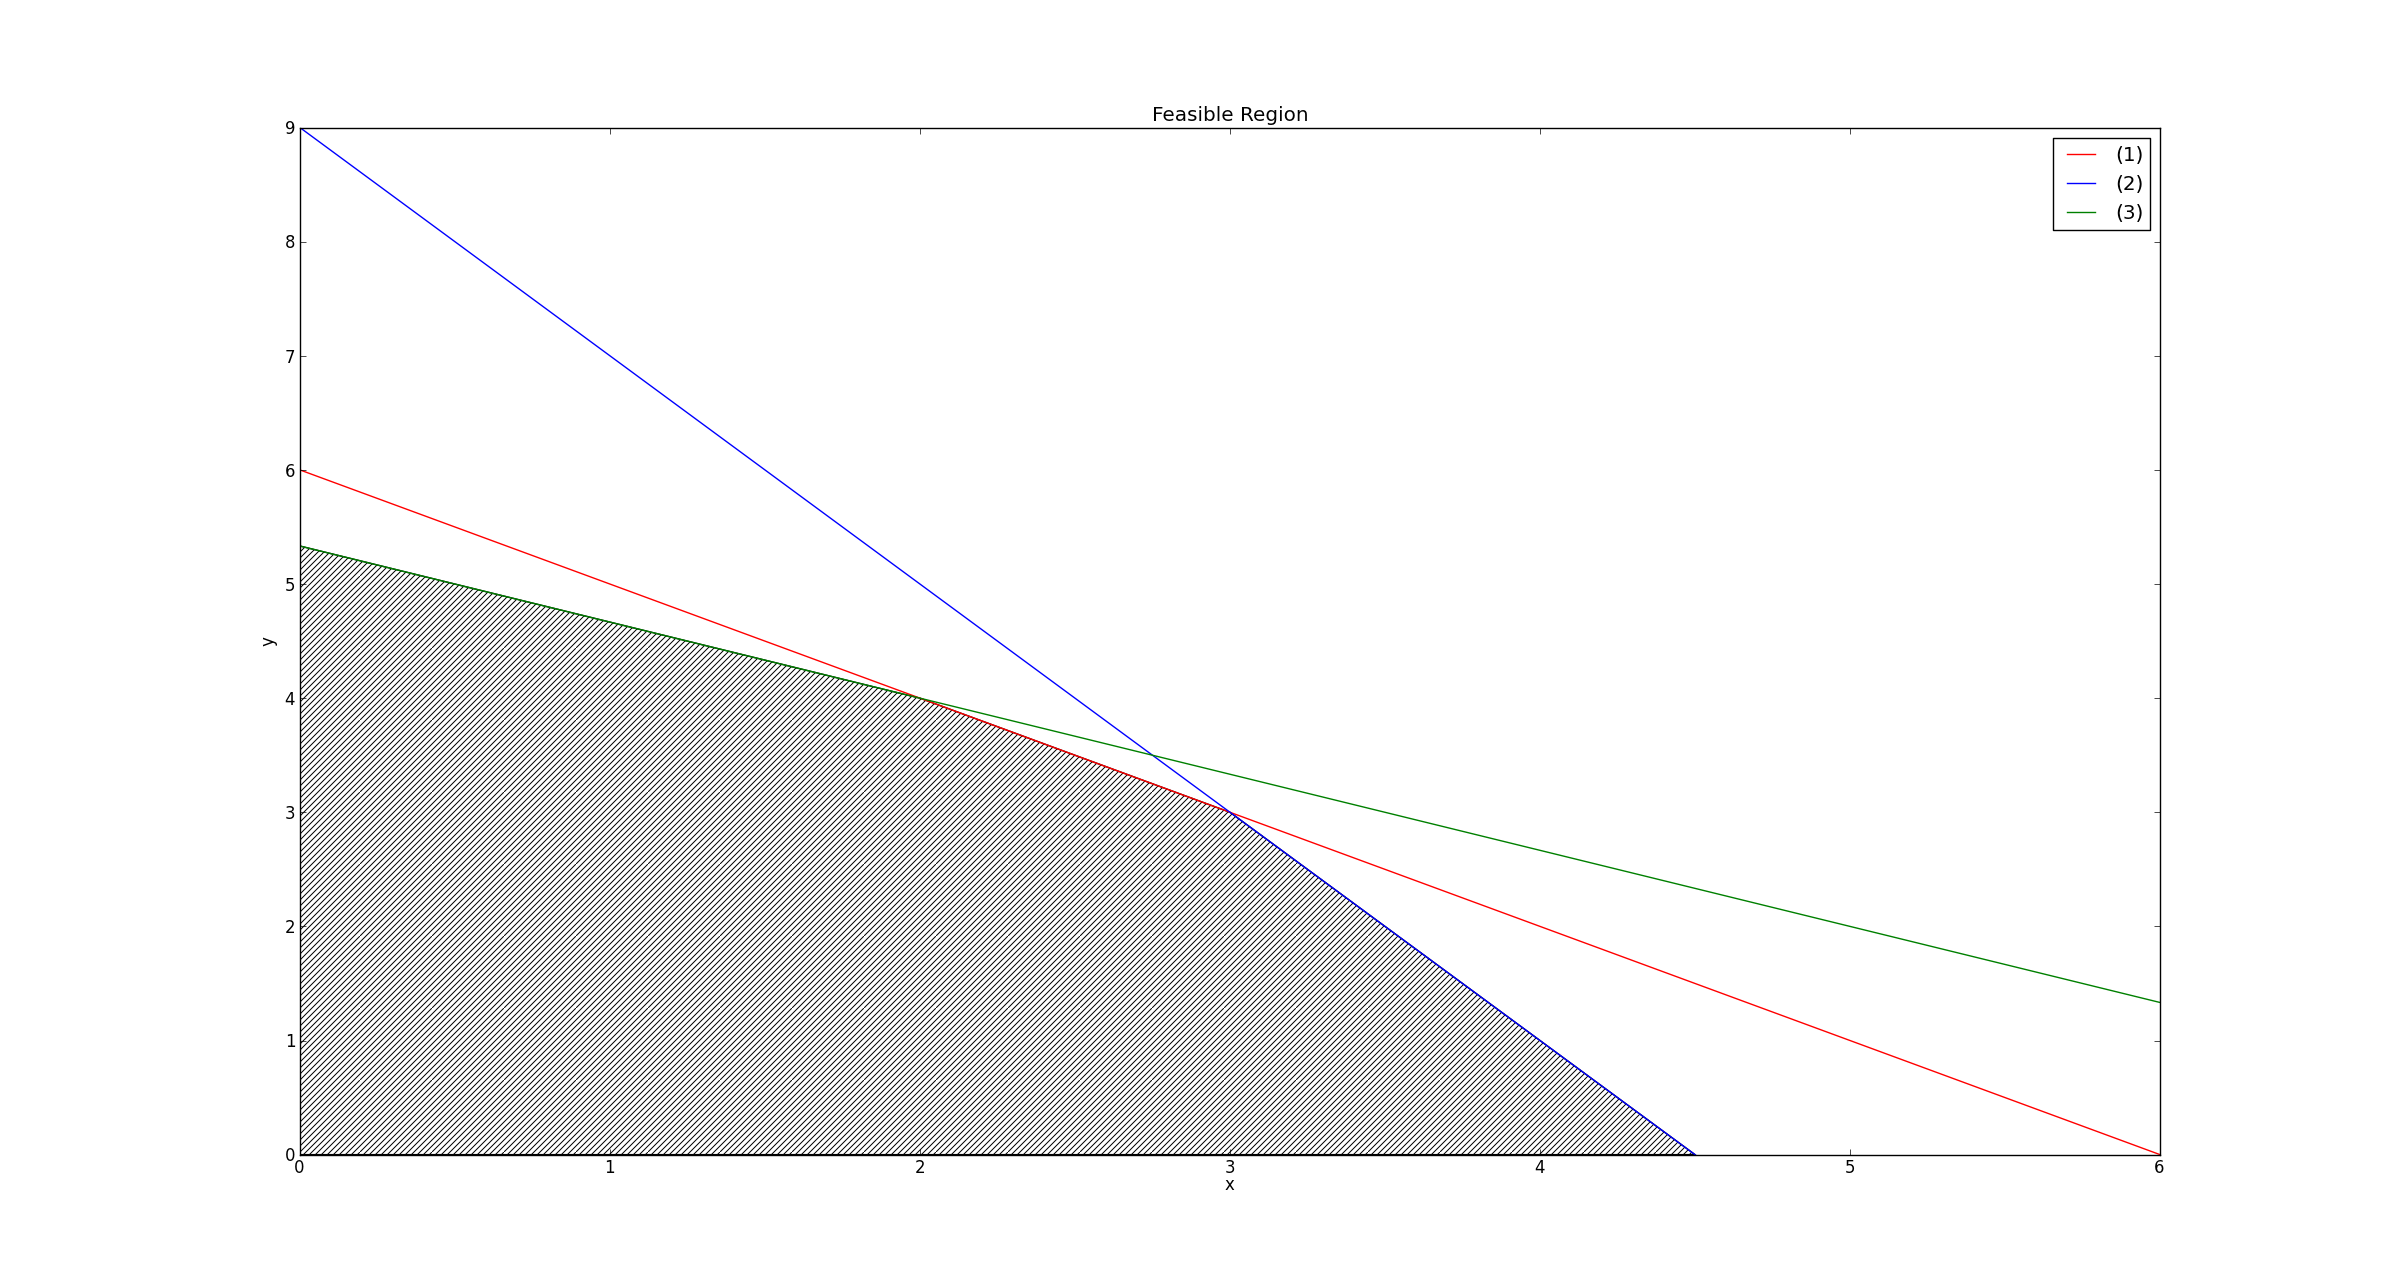
\includegraphics[scale=0.2]{feasible_region.png}
\end{frame}

\begin{frame}
\frametitle{Linear Programming Geometry}
\scriptsize
\begin{itemize}
\item Plot the objective function $z = 6x + 4y$ for some fixed values of $z$.
\item These are the so-called {\em isoprofit lines} or {\em objective function contours}.
\item Increasing $z$ results in a parallel shift to the right.
\end{itemize}
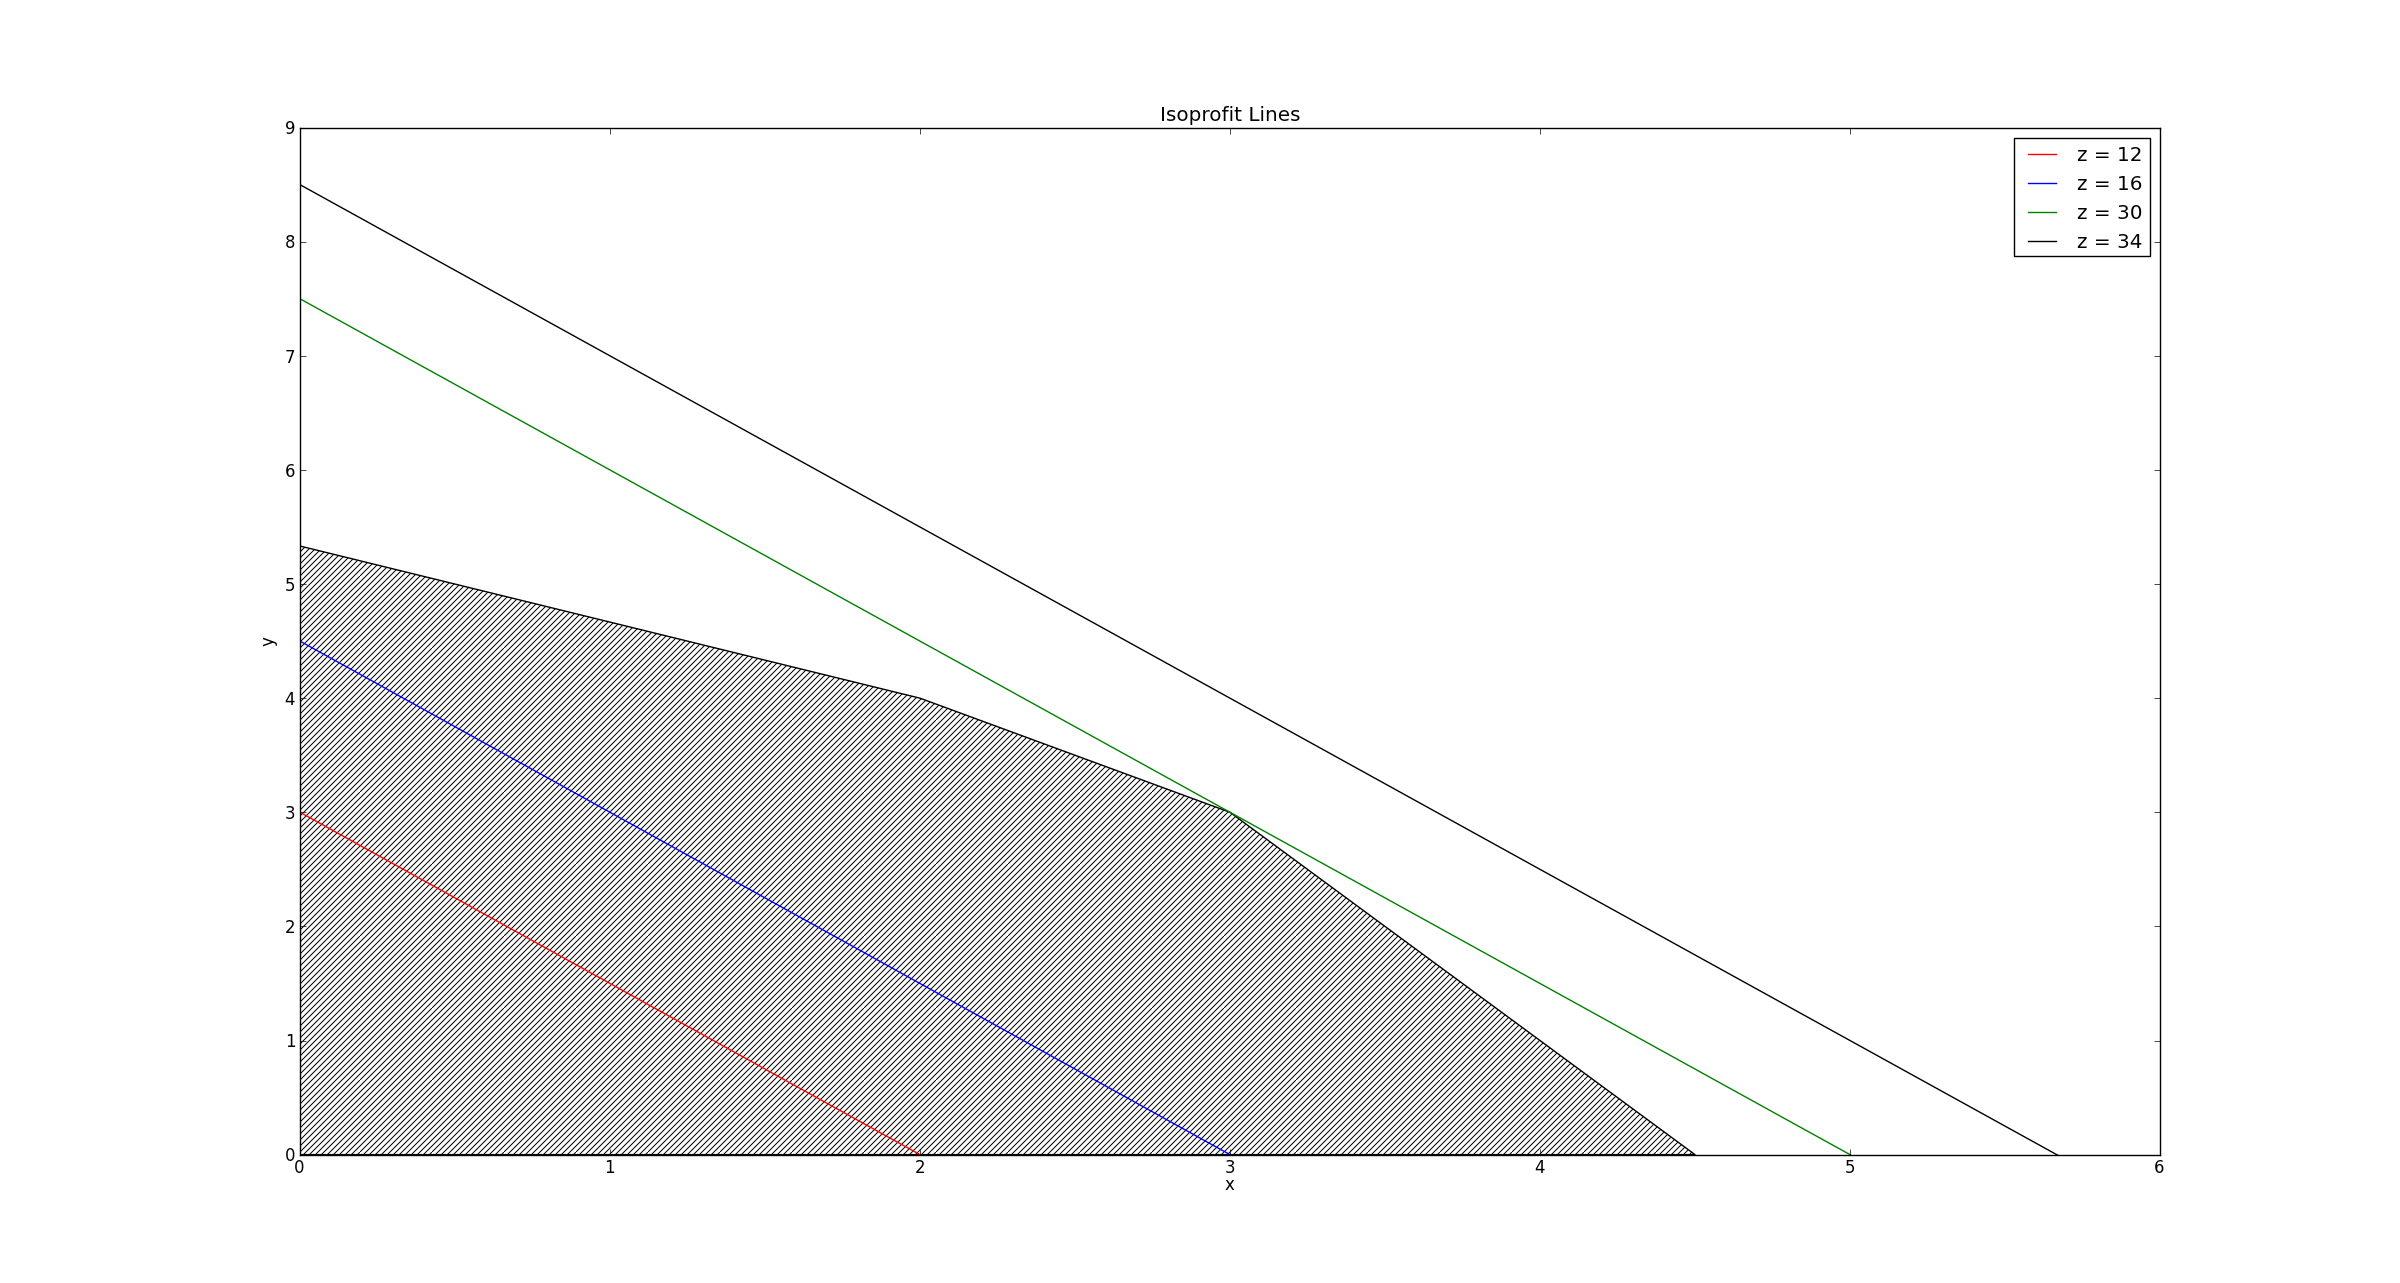
\includegraphics[scale=0.2]{isoprofit_lines.png}
\end{frame}

\begin{frame}
\frametitle{Observations}
\begin{itemize}
\item Feasible region of a linear program is always a convex polyhedron
\item At least one optimal solution occurs at a corner point (a.k.a. extreme point or vertex) of this polyhedron
\item Infinitely-many points in the feasible region, but only finitely many corner points
\end{itemize}
\end{frame}

\begin{frame}
\frametitle{Possible Outcomes of an LP}
\begin{itemize}
\item Infeasible - feasible region is empty, i.e., 
$x + 8y \ge 15$, $8x - y \le -1$, $x + y \ge -1$
\item Unbounded - no finite optimum, i.e. $x - y \le 10$ $2x + y \ge 10$
\item Multiple optima, i.e. $\mbox{max}\;\; 3x_1 + 3x_2$ subject to $x_1 + x_2 \le 1$ and non-negative
\item Unique optimal solution (as in previous example)
\end{itemize}
\end{frame}

\begin{frame}
\frametitle{Possible Outcomes of an LP}
\begin{itemize}
\item Infeasible - feasible region is empty, i.e., 
$x + 8y \ge 15$, $8x - y \le -1$, $x + y \ge -1$
\end{itemize}
\hfill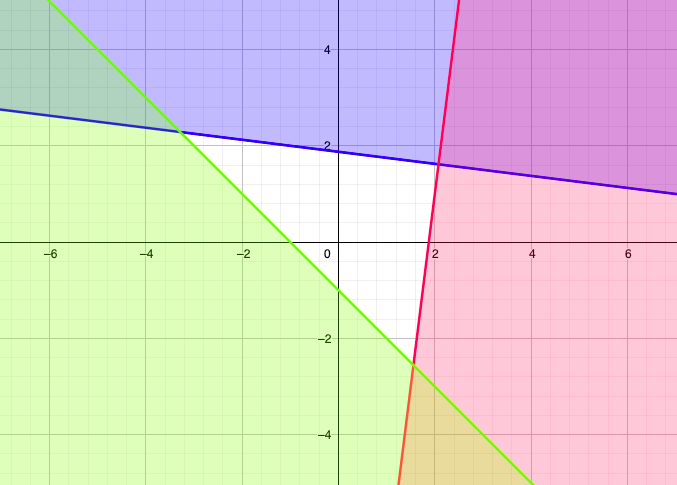
\includegraphics[scale=0.25]{infeasible.png}\hspace*{\fill}
\end{frame}

\begin{frame}
\frametitle{Possible Outcomes of an LP}
\begin{itemize}
\item Unbounded - no finite optimum, i.e. $\mbox{max}\;\;x+y$ subject to $x - y \le 10$, $2x + y \ge 10$
\begin{itemize}
\item Isoprofit lines can move outwards indefinitely
\end{itemize}
\end{itemize}
\hfill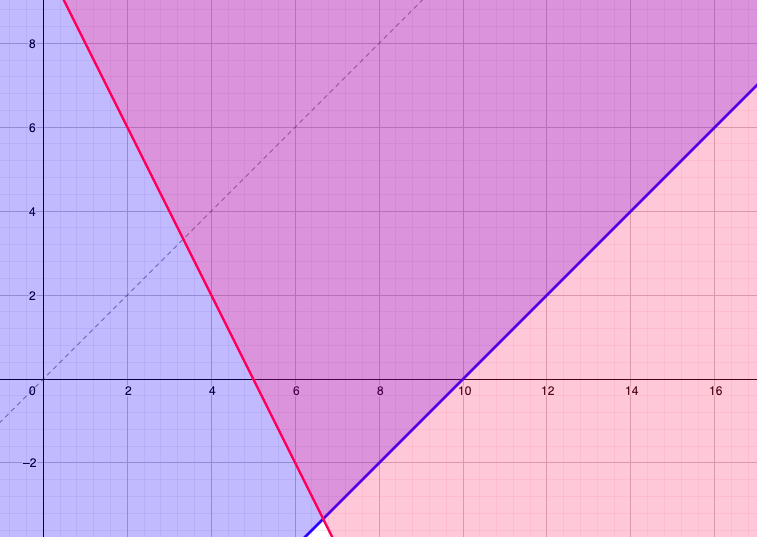
\includegraphics[scale=0.3]{unbounded.png}\hspace*{\fill}
\end{frame}

\begin{frame}
\frametitle{Linear Programming Solvers}
\begin{itemize}
  \item Finds {\em \bf an} optimal solution if feasible region is non-empty and objective function is bounded
  \item Might be multiple optimal solutions
  \begin{itemize}
    \item Which optimal solution returned is not defined.
  \end{itemize}
  \item Constraints are ``hard''
  \begin{itemize}
    \item Won't violate constraints \footnote{by more than the numerical tolerance} even if it helps the objective.
    \item Will tell if relaxing a constraint would help the objective.
  \end{itemize}
\item Solver makes no apologies for this behavior!
\item Includes proof of optimality
\end{itemize}
\end{frame}

\frame{\frametitle{Real Linear Programming Solvers}
Strengths
\begin{itemize}
  \item Can solve very large problems in practice
    \begin{itemize}
      \item Tuned for real-world business problems
      \item Routinely solve problems with $10^7$ variables and constraints
      \item Multiple algorithms (controlled by parameter Method)
    \end{itemize}
\end{itemize}
Weaknesses
\begin{itemize}
  \item Don't guarantee a time to a solution
  \item Might not reach optimality (but will tell you if it doesn't)
  \item Work with floating point values
  \begin{itemize}
    \item Might violate constraints by a small tolerance (controlled by parameter FeasibilityTol)
    \item Might return a solution that is within some numerical tolerance of optimal (controlled by parameter OptimalityTol)
  \end{itemize}
\end{itemize}
The better the linear programming solver,
the less of an issue you will have with these realities.
}

\begin{frame}
\frametitle{Notation}
Linear Programming involves exclusively addition and multiplication by constants.
The symbols $\in$ and $\notin$ is read as ``in'' and ``not in''.
If $I = \{1,2,3\}.$
\begin{block}{$$\sum_{i \in I} a_i x_i$$}
$$a_1 x_1 + a_2 x_2 + a_3 x_3$$
\end{block}
\begin{block}{$$x_i \le b_i \hspace{0.25in} \forall i \in I$$}
\begin{align*}
x_1 \le b_1 \\
x_2 \le b_2 \\
x_3 \le b_3 \\
\end{align*}
\end{block}
\end{frame}

\frame{\frametitle{Knapsack Problem}
\begin{itemize}
\item Set of items $I = \{1,\ldots,n\}$.
\item Each item has value $v_i$ and weight $w_i$.
\item Have a knapsack that with capacity $b$.
\item Can take part of any item.
\item What is the highest valued collection of items (and partial items) that can go into the knapsack?
\end{itemize}
\begin{eqnarray}
\max_x && \sum_{i \in I} v_i x_i \nonumber \\
\mbox{s.t.} && \sum_{i \in I} w_i x_i \le b \nonumber \\
&& 0 \le x_i \le 1,\;\;i \in I \nonumber
\end{eqnarray}
\begin{itemize}
\item Use a LinExpr to build up the sum in the constraint.
\end{itemize}
}

\begin{frame} [containsverbatim]
\frametitle{Python Implementation}
\scriptsize
\begin{verbatim}
import gurobipy as grb
weights = [70, 73, 77, 80, 82, 87, 90, 94, 98, 106, 110, 113, 115, 118, 120]
values = [135, 139, 149, 150, 156, 163, 173, 184, 192, 
201, 210, 214, 221, 229, 240]
capacity = 750
m = grb.Model()
item_selected = []
for i in range(len(values)):
    item_selected.append(m.addVar(ub=1, obj=values[i], 
    name=`item_selected.' + str(i)))
m.update()
total_weight = grb.quicksum(weights[i]*item_selected[i] 
for i in range(len(values)))
weight_con = m.addConstr(total_weight <= capacity, name=`total_weight')
m.update()
m.ModelSense = grb.GRB.MAXIMIZE
m.optimize()
for var in item_selected:
    print(var.VarName, var.X)
\end{verbatim}
\end{frame}

\frame{\frametitle{The Diet Problem Generalized}
\begin{itemize}
\item Sets and Indices
    \begin{itemize}
    \item $i \in I$: nutrients
    \item $j \in J$: food types
    \end{itemize}
\item Data
    \begin{itemize}
    \item $c_j$: per ounce cost of food type $j$
    \item $a_{ij}$: quantity of nutrient $i$ per ounce of food type $j$
    \item $l_i$, $u_i$: min, max daily requirements for nutrient $i$
    \end{itemize}
\item Decision Variables
    \begin{itemize}
    \item $x_j$: the number of ounces to consume of
 food type $j$.
    \end{itemize}
\item Formulation?
\item Let $\pi_i$ be the shadow price for nutrient $i$. What is the reduced cost of food type $j$, in terms of $\pi$?
\end{itemize}
}

\begin{frame} [containsverbatim]
\frametitle{Python Implementation}
Add ranged constraints to model via model.addRange(expr, lower, upper, name) \\
\tiny
\begin{verbatim}
def solve_diet_problem(nutrient_densities, costs, nutrient_requirements):
    m = grb.Model()
    ounces_consumed = {food_type: m.addVar(obj=cost, name=`ounces_consumed.' + str(food_type))
                       for food_type, cost in costs.iteritems()}
    m.update()
    nutrient_constraints = {}
    food_types = costs.keys()
    for nutrient, (min_requirement, max_requirement) in nutrient_requirements.iteritems():
        nutrient_consumed = grb.quicksum(nutrient_densities[food_type, nutrient]*ounces_consumed[food_type]
                                         for food_type in food_types)
        constr = m.addRange(nutrient_consumed, min_requirement, max_requirement,
                           `nutrient.' + str(nutrient))
        nutrient_constraints[nutrient] = constr
    m.optimize()
    if m.status == GRB.OPTIMAL:
        return {food_type: var.X for food_type, var in ounces_consumed.iteritems()}
    raise Exception("Model was infeasible.")
\end{verbatim}
\end{frame}

\begin{frame}
\frametitle{Transportation Problem}
\begin{center}
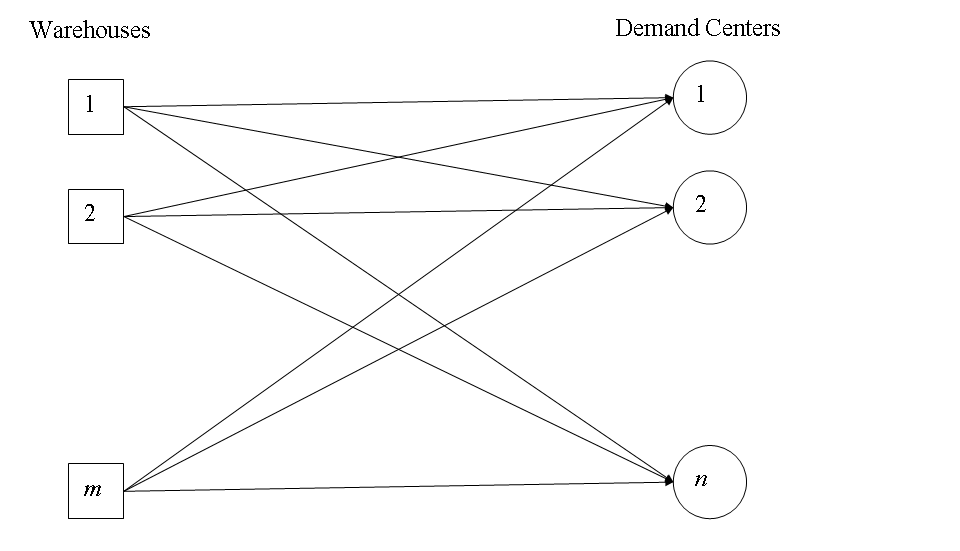
\includegraphics[scale = 0.3]{transportation_problem.png}
\end{center}
Input: \\
Warehouse capacity $u_i$ (widgets) \\
Customer demand $d_j$ (widgets) \\
Shipping cost $c_{ij}$ (\$/widget)
\end{frame}

\begin{frame}
\frametitle{Transportation Problem}
\begin{itemize}
\item Sets and Indices
    \begin{itemize}
    \item $i \in I$: Warehouses
    \item $j \in J$: Customers
    \end{itemize}
\item Data
    \begin{itemize}
    \item $u_i$: capacity for warehouse $i$ (widgets)
    \item $d_j$: demand at demand center $j$ (widgets)
    \item $c_{ij}$: shipping cost from warehouse $i$ to customer $j$ (\$/widget)
    \end{itemize}
\item Decision Variables
    \begin{itemize}
    \item $x_{ij}$: number of widgets to ship from warehouse $i$ to customer $j$
    \end{itemize}
\end{itemize}
\end{frame}

\begin{frame}
\frametitle{LP Formulation}
\begin{eqnarray}
\min_{x} && \sum_{i \in I} \sum_{j \in J} c_{ij} x_{ij} \;\; \mbox{(minimize shipping costs)} \nonumber \\
\mbox{s.t.} && \sum_{i \in I} x_{ij} = d_j,\;\;j \in J \;\; \mbox{(satisfy demand)}\nonumber \\
&& \sum_{j \in J} x_{ij} \le u_i,\;\;i \in I \;\; \mbox{(don't exceed capacity)} \nonumber \\
&& x_{ij} \ge 0, \;\;i \in I,\;j \in J \;\; \mbox{(ship nonnegative quantities)} \nonumber
\end{eqnarray}
\end{frame}

\begin{frame} [containsverbatim]
\frametitle{Python Implementation}
Use quicksum to build up the summations in the constraints. \\
Assume $to\_ship$ is a 2d array of vars and has already been populated. \\
Demand constraints $\sum_{i \in I} x_{ij} = d_j,\;\;j \in J$ are built via: \\
{\scriptsize
\begin{verbatim}
def get_demand_constrs(model, to_ship, demands):
    return [model.addConstr(grb.quicksum(to_ship[warehouse, customer] 
                            for warehouse in warehouses) == demand, 
                            name=`demand.' + str(customer))
           for customer, demand in enumerate(demands)]
\end{verbatim}
}

Capacity constraints $\sum_{j \in J} x_{ij} \le u_i,\;\;i \in I$ are built via: \\
{\scriptsize
\begin{verbatim}
def get_capacity_constrs(model, to_ship, capacities):
    return [model.addConstr(grb.quicksum(to_ship[warehouse, customer] 
                            for customer in customers) <= capacity, 
                            name=`capacity.' + str(warehouse))
            for warehouse, capacity in enumerate(capacities)]
\end{verbatim}
\end{frame}
}
\begin{frame}
\frametitle{Diagnosing Infeasibility}
\begin{itemize}
\item After optimization, always check the Model attribute Status to determine whether the model was solved to optimality.
\item If model is infeasible, Status will be GRB.Status.Infeasible
\item model.computeIIS() computes an irreducible inconsistent subsystem.
\item Pass model.write() a filename with suffix .ilp to write the IIS to a file.
\item Var attributes IISLB, IISUB indicate which variable bounds participate in the IIS.
\item Constr attributes IISConstr indicate which constraints participate in the IIS.
\end{itemize}
\end{frame}

{
\setbeamercolor{background canvas}{bg=exerciseblue}
\begin{frame}
\frametitle{Exercise}
\begin{itemize}
\item Implement the transportation model with Gurobi.
\item Under what conditions would the problem become infeasible?
\item Create an infeasible instance, compute an IIS, and write it to a file.
\end{itemize}
\end{frame}
}

\begin{frame}
\frametitle{Elasticizing Constraints}
To extend the transportation problem allow demand to go unsatisfied at a per-unit penalty of $\rho$ replace the demand constraint with
\begin{equation}
\sum_{i \in I} x_{ij} = d_j - y_j,\;\;j \in J, \nonumber
\end{equation}
\noindent where $y_j \ge 0$, and add $\rho \sum_{j \in J} y_j$ to the objective.
\end{frame}

\begin{frame}
\frametitle{Piecewise Linear Penalties}
Penalize the first 20\% of demand shortfall at a rate $\rho$, and any additional demand shortfall at a rate $1.5\rho$.
\begin{eqnarray}
\sum_{i \in I} x_{ij} = d_j - y_j^1 - y_j^2,\;\;j \in J \nonumber \\
0 \le y_j^1 \le 0.2d_j,\;\;j \in J \nonumber \\
0 \le y_j^2,\;\;j \in J, \nonumber
\end{eqnarray}
\noindent and add $\rho \sum_{j \in J} (y_j^1 + 1.5 y_j^2)$ to the objective.


\end{frame}

\begin{frame}
\frametitle{Piecewise Linear Penalties}
\begin{itemize}
\item Starting with 6.0, Gurobi provides a method model.setPWLObj.
\end{itemize}
\begin{center}
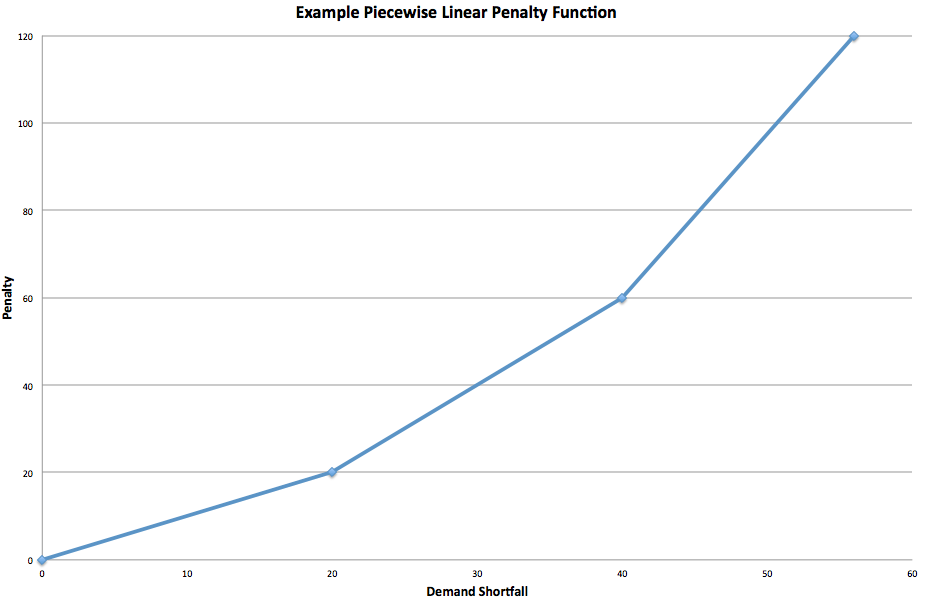
\includegraphics[scale=0.2]{piecewise_linear.png}
\end{center}
\begin{itemize}
\item The above penalty function can be created in one call:
\begin{itemize}
\item model.setPWLObj(var, [0, 20, 40, 56], [0, 20, 60, 120])
\end{itemize}
\item No auxiliary variables are required.
\item Note: If the objective function is not convex, the resulting model will be an Integer Program.
\end{itemize}
\end{frame}

\begin{frame}
\frametitle{Minimize the Maximum Demand Shortfall}
\begin{itemize}
\item Recall: $\sum_{i \in I} x_{ij} = d_j - y_j,\;\;j \in J$
\item $y_j$ is the demand shortfall at demand center $j$.
\item Suppose we want to control $z = \max \{y_1, y_2, \ldots, y_n\}$.
\item Let $z \ge y_j,\;\;j \in J$.
\item Penalize $z$ in the objective, or put an upper bound on $z$.
\item Only works if we are trying to minimize $z$, otherwise we require integer variables.
\item Extends to any problem involving minimization (maximization) of the maximum (minimum) of several linear functions.
\item $y = |x|$ can be linearized as $y \ge x$, $y \ge -x$ (assuming minimization of $y$).
\end{itemize}
\end{frame}

\begin{frame}
\frametitle{Multiple Objectives}
\begin{eqnarray}
\min_{x} && \sum_{i \in I} \sum_{j \in J} c_{ij} x_{ij} + \rho \sum_{j \in J} y_j \nonumber \\
\mbox{s.t.} && \sum_{i \in I} x_{ij} = d_j - y_j,\;\;j \in J \nonumber \\
&& \sum_{j \in J} x_{ij} \le u_i,\;\;i \in I \nonumber \\
&& x_{ij} \ge 0, \;\;i \in I,\;j \in J \nonumber \\
&& y_j \ge 0,\;\;j \in J \nonumber \end{eqnarray}
\begin{itemize}
\item Objectives:
    \begin{itemize}
    \item Minimize transportation cost $\sum_{i \in I} \sum_{j \in J} c_{ij} x_{ij}$
    \item Minimize demand shortfall $\sum_{j \in J} y_j$
    \end{itemize}
\item How do we choose $\rho$?
\end{itemize}
\end{frame}

\begin{frame}
\frametitle{Multiple Objectives}
\begin{itemize}
\item Generate an {\em efficient frontier} of solutions.
\item Let $z = \sum_{j \in J} y_j$.
\item Add $\rho z$ to the objective.
\item Optimize with $\rho = 0$.
\item Query Var attribute SAObjUp.
\item Reoptimize with $\rho = (1+\epsilon)\mbox{SAObjUp}$.
\item LPs are cheap to reoptimize!
\end{itemize}
\end{frame}

{
\setbeamercolor{background canvas}{bg=exerciseblue}
\begin{frame}
\frametitle{Exercise}
Generate the efficient frontier of the transportation problem.
\end{frame}
}

\begin{frame} [containsverbatim]
\frametitle{Primary and Secondary Objectives}
\begin{itemize}
\item Optimize primary objective first.
\item Constrain primary objective to be within some tolerance of optimal.
\item Optimize secondary objective.
\end{itemize}
\small
\begin{verbatim}
primary = grb.LinExpr()
secondary = grb.LinExpr()
// build up objective functions
m.setObjective(primary)
m.optimize()
objValue = model.objVal
m.addConstr(primary, `L', (1 + EPS)*objValue, "PrimaryObj")
m.setObjective(secondary)
m.optimize()
\end{verbatim}
\end{frame}

\begin{frame}
\frametitle{Best Modeling Practices}
\begin{itemize}
\item Allow objectives to become constraints and vice versa
\item Multiple optima are the norm, not the exception
    \begin{itemize}
    \item Exploit this with tie-breakers (secondary, tertiary objectives)
    \end{itemize}
\item Elasticize constraints
\end{itemize}
\end{frame}

\frame{\frametitle{Shortest Path}
\begin{itemize}
\item Let $N$ be a set of cities.
\item Let $A$ be a set of arcs between cities.
\item Let $d_{ij}$ be the distance between city $i \in N$ and city $j \in N$.
\item What is the shortest distance between a given origin city $s \in N$ and destination city $t \in N$?
\end{itemize}
\begin{center}
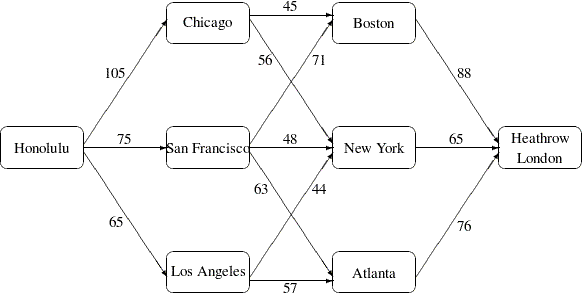
\includegraphics[scale=0.5]{netflow.png}
\end{center}
}

\begin{frame}
\frametitle{Shortest Path}
Let $x_{ij} = 1$ if arc $(i,j)$ is traversed.
\begin{eqnarray}
\min_x && \sum_{(i,j) \in A} d_{ij} x_{ij} \nonumber \\
\mbox{s.t.} && \sum_{j \in RS(i)} x_{ji} - \sum_{j \in FS(i)} x_{ij} = b_i,\;\;i \in N \nonumber \\
&& 0 \le x_{ij} \le 1,\;\;(i,j) \in A, \nonumber
\end{eqnarray}
\noindent where $FS(i) = \{j | (i,j) \in A\}$, $RS(i) = \{j | (j, i) \in A\}$, $b_s = -1$, $b_t = 1$, and $b_i = 0$ for $i \neq s, t$.
\end{frame}

\end{document}

\begin{frame}
\frametitle{Shortest Path}
\begin{itemize}
\item Let $\pi_j$ be the length of the shortest path from the origin to city $j$.
\item Can write $\pi_j = \min_{(i,j) \in A} d_{ij} + \pi_i$ for every $j \in N$.
\item Linearize, and maximize $\pi_t$ to compute length of shortest path.
\item Tight constraints indicate arcs on the shortest path.
\end{itemize}
\begin{eqnarray}
\max_{\pi} && \pi_t \nonumber \\
\mbox{s.t.} && \pi_j \le \pi_i + d_{ij},\;\;(i,j) \in A \nonumber \\
&& \pi_s = 0 \nonumber
\end{eqnarray}
\end{frame}

{
\setbeamercolor{background canvas}{bg=exerciseblue}
\begin{frame}
\frametitle{Exercise}
Implement both shortest path formulations. How are the two formulations related?
\end{frame}
}
